%!TeX root=../tese.tex

\chapter{Literatura Cinzenta}
\label{cap:literatura-cinzenta}

Literatura cinzenta é o nome dado para publicações, textos e produções os quais não passaram pelo mesmo processo de revisão por pares que a chamada literatura branca, que inclui, por exemplo, publicações formais, artigos científicos e periódicos. Neste capítulo, estão listados os relatórios de literatura cinzenta utilizados na pesquisa 

\section{GitClear — AI Copilot Code Quality: Evaluating 2024's Increased Defect Rate via Code Quality Metrics}
Este relatório foi escrito pela empresa GitClear, que desenvolve ferramentas de análise de código-fonte para empresas de desenvolvimento de software. O relatório realizou uma análise de métricas de qualidade de código de 211 milhões de linhas alteradas em 2024, sendo dois terços destas linhas advindos do compartilhamento de dados anonimizados de empresas privadas e o restante de projetos de código livre. Os pesquisadores criaram um histórico comparando as métricas observadas em pesquisas anteriores com as métricas de 2024 e a análise é feita com foco no impacto de ferramentas de IA generativa no processo de desenvolvimento de software, considerando 2022 como o ano em que a ampla adoção da IA na programação se iniciou.

\begin{table}[h]
\centering
\footnotesize
\caption{Histórico de métricas de código de 2020 a 2024 (\cite{gitclear2025}).}
\label{tab:historico_metricas}
\setlength{\tabcolsep}{6pt}
\renewcommand{\arraystretch}{1.2}

\begin{tabular}{llllllll}
	\toprule
	Ano & Adicionado & Deletado & Atualizado &
	Movido & Cópia & Substituído & Churn \\
	\midrule
	2020 & 39,2\% & 19,1\% & 5,2\% & 24,1\% & 8,3\% & 2,9\% & 3,1\% \\
	2021 & 39,5\% & 19,3\% & 5,0\% & 24,8\% & 8,4\% & 3,4\% & 3,3\% \\
	2022 & 40,9\% & 19,8\% & 5,2\% & 20,5\% & 9,4\% & 3,7\% & 3,3\% \\
	2023 & 42,3\% & 21,1\% & 5,6\% & 15,8\% & 10,6\% & 3,6\% & 4,5\% \\
	% \rowcolor{gray!15}
	% 2024 Projected & 43,6\% & 22,1\% & 5,8\% & 13,4\% & 11,6\% & 3,6\% & 7,1\% \\
	2024 & 46,2\% & 21,9\% & 5,9\% & \cellcolor{red!15} 9,5\% & \cellcolor{red!15} 12,3\% & 4,2\% & \cellcolor{red!15} 5,7\% \\
	% \rowcolor{yellow!20}
	% YoY change & +9,2\% & +3,8\% & +7,2 & -39,9\% & +17,1\% & +16,7\% & +26\%
	\bottomrule
\end{tabular}
\end{table}

Na tabela \autoref{tab:historico_metricas}, são apresentados os resultados das análises entre 2020 e 2024. Observa-se que a porcentagem de linhas movidas, algo associado a refatorações estruturais, reorganização de trechos e melhorias arquiteturais, apresentou uma queda significativa, passando de 24,1\% em 2020 para apenas 9,5\% em 2024. Por outro lado, a tendência para as linhas copiadas foi inversa, partindo de 8,3\% em 2020 para 12,3\% em 2024. Este aumento de duplicações também pode ser observado na \autoref{tab:duplicacao_codigo}, que mostra que, em 2020, apenas 0,7\% dos commits analisados continham blocos de código duplicados e, em 2024, esse número subiu para 6,66\%.

\begin{table}[h!]
	\centering
	\footnotesize
	\caption{Histórico de duplicação de código nos commits de 2020 a 2024 (\cite{gitclear2025}).}
	\label{tab:duplicacao_codigo}
	\setlength{\tabcolsep}{8pt}
	\renewcommand{\arraystretch}{1.2}
	\begin{tabular}{l l l l l}
		\toprule
		Ano &
		Tot. commits &
		Tot. duplicações &
		Commits com duplicação &
		Commits com duplicação (\%) \\
\midrule
2020 & 19{.}805 & 9{.}227 & 139 & 0,70\% \\
2021 & 29{.}912 & 9{.}295 & 143 & 0,48\% \\
2022 & 40{.}010 & 10{.}685 & 182 & 0,45\% \\
2023 & 41{.}561 & 20{.}448 & 747 & 1,80\% \\
2024 & 56{.}495 & 63{.}566 & 3{.}764 & 6,66\% \\
\bottomrule
\end{tabular}
\end{table}

Além disso, outra métrica relevante neste contexto é o \emph{churn}, que busca medir quanto retrabalho é efetuado em uma base de código. Neste relatório, o \emph{churn} é calculado medindo quanto das linhas escritas e enviadas ao repositório foram revertidas ou substancialmente revisadas nas duas semanas seguintes. A \autoref{tab:historico_metricas} mostra que o \emph{churn} passou de 3,1\% em 2020 para 5,7\% em 2024, evidenciando o aumento do retrabalho no código.

O relatório fez também uma análise de quanto tempo se passou entre o momento em que os códigos analisados foram criados e em quanto tempo eles receberam sua próxima mudança significativa. Na \autoref{fig:historico_tempo_mudanca}, observa-se que a proporção de linhas que em menos de duas semanas foram alteradas aumentou de 60,4\% em 2020 para 69,7\% em 2024, em contrapartida, o grupo das linhas que precisaram de alterações apenas depois de 4 semanas, mas antes de um ano, diminuiu de 24,7\% para 16,9\% no mesmo período.

Desta maneira, o relatório conclui que houve aumento da duplicação de linhas nos repositórios, violando a boa prática DRY (\emph{Don't Repeat Yourself}), a diminuição da proporção de linhas movidas, que indicam refatoração, o aumento da instabilidade do código, já que o \emph{churn} aumentou, e uma redução da durabilidade do código, no sentido dele precisar ser reescrito ou modificado mais cedo. O relatório credita este cenário de piora da qualidade do código e de sua manutenibilidade no longo prazo à adoção de IA no desenvolvimento de \emph{software}.

\begin{figure}[h!]
\caption{Proporção anual das linhas modificadas classificadas pelo tempo que permaneceram no repositório antes de sofrerem uma nova modificação significativa entre 2020 e 2024 (\cite{gitclear2025}).}
\centering
\label{fig:historico_tempo_mudanca}

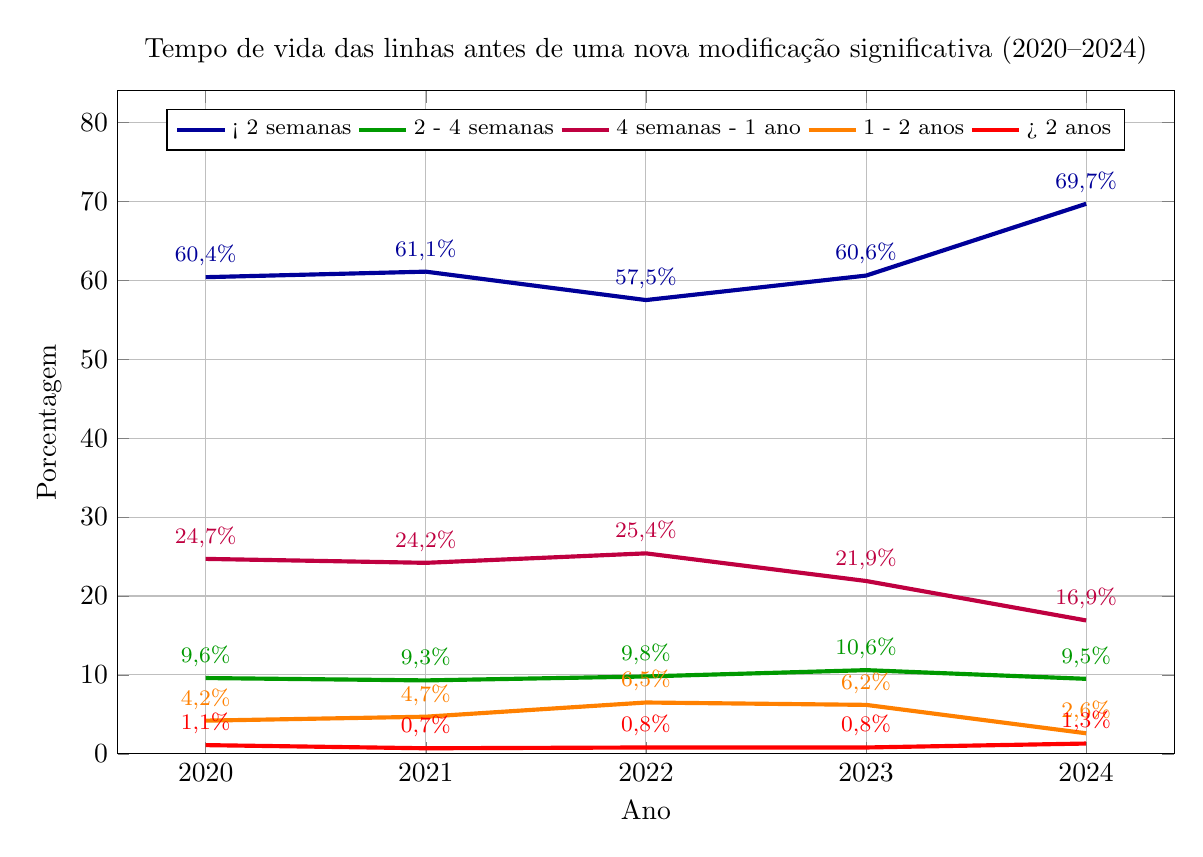
\begin{tikzpicture}
\begin{axis}[
	/pgf/number format/use comma,
    every axis plot/.style={ line width=1.5pt },
    width=15cm,
    height=10cm,
    xlabel={Ano},
    ylabel={Porcentagem},
    title={Tempo de vida das linhas antes de uma nova modificação significativa (2020–2024)
},
    ymin=0,
    ymax=84,
    legend style={
        font=\footnotesize,
        at={(0.5,0.91)},
        anchor=south,
        legend columns=5,
    },
    grid=both,
    symbolic x coords={2020,2021,2022,2023,2024},
    xtick=data,
    nodes near coords={\pgfmathprintnumber{\pgfplotspointmeta}\%},
    every node near coord/.append style={
        font=\footnotesize,
        anchor=south,
    },
]

\addplot[color=blue!60!black] coordinates {
    (2020,60.4) (2021,61.1) (2022,57.5) (2023,60.6) (2024,69.7) 
};
\addlegendentry{< 2 semanas}

\addplot[color=green!60!black] coordinates {
    (2020,9.6) (2021,9.3) (2022,9.8) (2023,10.6) (2024,9.5)
};
\addlegendentry{2 - 4 semanas}

\addplot[color=purple] coordinates {
    (2020,24.7) (2021,24.2) (2022,25.4) (2023,21.9) (2024,16.9)
};
\addlegendentry{4 semanas - 1 ano}

\addplot[color=orange] coordinates {
    (2020,4.2) (2021,4.7) (2022,6.5) (2023,6.2) (2024,2.6)
};
\addlegendentry{1 - 2 anos}

\addplot[color=red] coordinates {
    (2020,1.1) (2021,0.7) (2022,0.8) (2023,0.8) (2024,1.3)
};
\addlegendentry{> 2 anos}

\end{axis}
\end{tikzpicture}

\end{figure}



\section{Stack Overflow: Developer Survey}
Esta pesquisa foi realizada pelo \emph{Stack Overflow}, plataforma reconhecida no campo de tecnologia como meio de encontrar respostas para dúvidas relacionadas a códigos, linguagens de programação, \emph{frameworks}, algoritmos e tecnologias em geral. O \emph{Stack Overflow} realiza desde XXXX uma pesquisa anual aberta com usuários do sistema de modo a levantar dados sobre as tendências no mercado de tecnologia, impressões dos desenvolvedores, entre outros. Os entrevistados incluem desde programadores profissionais experientes até pessoas que estão iniciando seus estudos sobre programação.  

Os resultados da pesquisa em 2024 incluem uma seção específica para tratar a IA e seus impactos no mercado. Dentre os respondentes, 61,8\% utiliza ferramentas de IA em seus processos de desenvolvimento de código e outros 13,8\% planeja utilizar, além disso, 72\% é favorável ou muito favorável ao uso de IA.

		43% confia na precisão da IA e 30,4% não confia
		43,2% acredita que a IA é ruim ou péssima lidando com tarefas complexas
		68,3% acredita que a IA não é uma ameaça a seus trabalhos
		
	Descrição do uso
		Benefícios
		Principais usos



\section{Gartner: Principais Tendências Tecnológicas Estratégicas para 2025: IA Agêntica}
Este relatório

\section{Gartner: Magic Quadrant for AI Code Assistants}
Este relatório

% Teses e dissertações, anais de conferências, boletins informativos, relatórios, documentos governamentais e parlamentares, comunicações informais, traduções, dados de censo, relatórios de pesquisa, relatórios técnicos, padrões, patentes, vídeos, ensaios clínicos e diretrizes práticas, eprints, preprints, artigos wiki, e-mails, blogs, arquivos de dados de pesquisa e dados científicos, levantamentos geológicos e geofísicos, mapas, conteúdo de repositórios.

